\chapter{Определение положения плоскости}\label{ch:ch1}
\setcounter{kiselevparagraph}{343} % Первый пункт главы в издании 1914 года — 344.

% А. П. Киселёв, «Элементарная геометрия», 23-е издание, 1914. Печатные с. 271–275.
% Печатная с. 271.
\kiselevparagraph{para:plane-definition} \textbf{Определение.} Плоскостью (\hyperref[para:intro-plane]{см.~Введение, пункт~\ref*{para:intro-plane}}) называется поверхность, обладающая тем свойством, что прямая, проходящая через две произвольные точки этой поверхности, \emph{целиком лежит на этой поверхности}. Возможность существования такой поверхности принимается за аксиому.

\emph{Стереометрией} (\hyperref[para:intro-branches-of-geometry]{см.~Введение, пункт~\ref*{para:intro-branches-of-geometry}}) называется часть геометрии, в которой рассматриваются свойства фигур, не все части которых лежат в одной плоскости.

\kiselevparagraph{para:plane-axioms} \textbf{Аксиомы плоскости.} Укажем следующие свойства плоскости, которые мы принимаем за очевидные:

\begin{enumerate}[label=\arabic*),ref=\arabic*]
    \item Плоскость --- \emph{незамкнутая} поверхность.
    \item Любая плоскость делит пространство на две части, расположенные по разные стороны от неё.
    \item\label{item:line-crosses-plane} Прямая, имеющая с плоскостью только одну общую точку, \emph{пересекает} плоскость, т.~е. из части пространства, лежащей по одну сторону от плоскости, переходит в часть пространства, лежащую по другую её сторону; поэтому две полупрямые, на которые плоскость делит эту прямую, лежат по разные стороны от неё.
    % Печатная с. 272.
    \item\label{item:segment-crosses-plane} Отрезок прямой, соединяющий две точки пространства, расположенные по разные стороны от плоскости, \emph{пересекает} эту плоскость, тогда как отрезок прямой, соединяющий две точки, расположенные по одну сторону плоскости, не пересекает её.
    \item Через любую прямую можно провести \emph{бесчисленное множество} плоскостей.
    \item Любая прямая на плоскости делит её на две части (называемые \emph{полуплоскостями}).
    \item Плоскость можно вращать вокруг любой прямой, лежащей на ней, причём каждую из частей, на которые плоскость делится этой прямой, можно заставить пройти через любую точку пространства.
\end{enumerate}

\kiselevparagraph{para:plane-representation} \textbf{Изображение и обозначение плоскости.} На рисунке изображают часть плоскости, обычно в форме параллелограмма или прямоугольника (рис.~\ref{fig:kiselev-stereo-301}). Плоскость обычно обозначают одной или двумя буквами, например: плоскость \(P\), плоскость \(MN\).

\begin{figure}[htbp]
    \centering
    \renewcommand{\thefigure}{301}
    \captionsetup{name=Рис.,labelsep=period}
    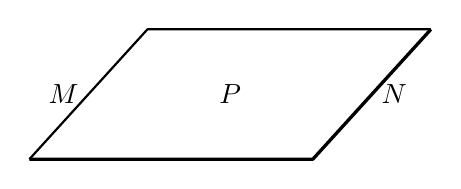
\begin{tikzpicture}[line join=round]
    \coordinate (front left) at (0,0);
    \coordinate (front right) at (3.6,0);
    \coordinate (back left) at (1.5,1.65);
    \coordinate (back right) at (5.1,1.65);

    \draw[thick] (front left) -- (back left) -- (back right);
    \draw[very thick] (front left) -- (front right) -- (back right);
    \path (front left) -- (back left) node[midway,left] {\(M\)};
    \path (front right) -- (back right) node[midway,right] {\(N\)};
    \node at (2.55,0.825) {\(P\)};
\end{tikzpicture}

    \caption{Изображение и обозначение плоскости}\label{fig:kiselev-stereo-301}
\end{figure}

\kiselevparagraph{para:plane-through-three-points} \textbf{Теорема. Через любые три точки} (\(A\), \(B\) и \(C\), рис.~\ref{fig:kiselev-stereo-302}), \textbf{не лежащие на одной прямой, можно провести ровно одну плоскость.}

\begin{figure}[htbp]
    \centering
    \renewcommand{\thefigure}{302}
    \captionsetup{name=Рис.,labelsep=period}
    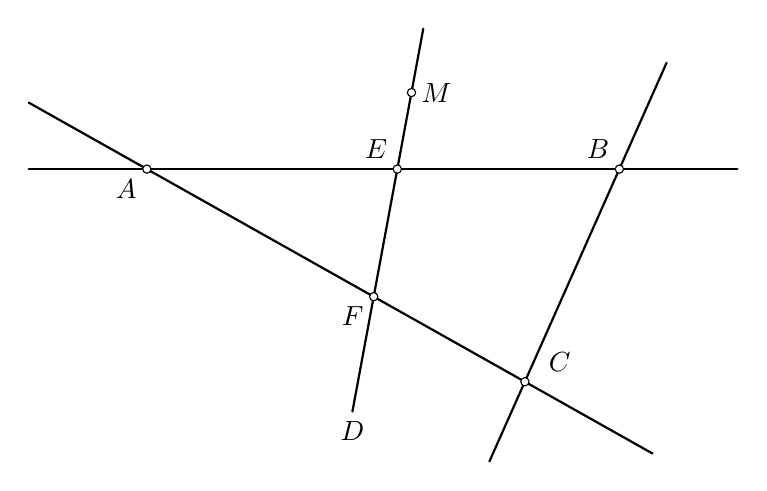
\begin{tikzpicture}[scale=1.5,line cap=round,every node/.style={inner sep=3.5pt}]
    \coordinate (A) at (0,0);
    \coordinate (B) at (4,0);
    \coordinate (C) at (3.2,-1.8);
    \coordinate (D) at (1.74,-2.052);
    \coordinate (E) at (2.12,0);
    \coordinate (F) at (1.92,-1.08);
    \coordinate (M) at (2.24,0.648);

    \draw[thick] (-1,0) -- (5,0);
    \draw[thick] (-1,0.5625) -- (4.28,-2.4075);
    \draw[thick] (4.4,0.9) -- (2.9,-2.475);
    \draw[thick] (2.34,1.188) -- (D);

    \foreach \point/\placement in {A/below left,B/above left,E/above left,F/below left,M/right} {
        \filldraw[fill=white] (\point) circle[radius=1pt] node[\placement] {\(\point\)};
    }
    \filldraw[fill=white] (C) circle[radius=1pt] node[above right,xshift=5pt] {\(C\)};
    \node[below] at (D) {\(D\)};
\end{tikzpicture}

    \caption{Плоскость, которая проходит через три точки \(A\), \(B\) и \(C\)}\label{fig:kiselev-stereo-302}
\end{figure}

\begin{enumerate}[label=\arabic*)]
    \item Через две любые из трёх данных точек, например через \(A\) и \(B\), проведём прямую, а через неё --- произвольную плоскость. Будем вращать эту плоскость вокруг прямой \(AB\), пока она не пройдёт через точку \(C\). Получим плоскость, которая проходит через три точки \(A\), \(B\) и \(C\).

    Остаётся доказать, что такая плоскость может быть только одна.

    \item Предположим, что через те же три точки проведены две плоскости. Обозначим одну \(P\), а другую --- \(P_1\).
    % Печатная с. 273.
    Докажем, что эти плоскости сливаются в одну. Сначала заметим, что прямые \(AB\), \(BC\) и \(AC\), проходящие через каждую пару данных точек, принадлежат обеим плоскостям, так как эти прямые имеют по две общие точки и с плоскостью \(P\), и с плоскостью \(P_1\). Теперь возьмём на плоскости \(P\) произвольную точку \(M\) и докажем, что эта точка принадлежит и другой плоскости \(P_1\). Для этого на плоскости \(P\) через точку \(M\) проведём прямую \(MD\) так, чтобы она пересекала \(AB\) и \(AC\) в точках \(E\) и \(F\). Так как прямые \(AB\) и \(AC\) принадлежат и другой плоскости \(P_1\), то их точки \(E\) и \(F\) также принадлежат этой плоскости. Поэтому прямая \(MD\), проходящая через \(E\) и \(F\), целиком лежит в плоскости \(P_1\) (\hyperref[para:plane-definition]{по определению плоскости}), а значит, и её точка \(M\) лежит в этой плоскости. Таким образом, любая точка \(M\) плоскости \(P\) принадлежит и плоскости \(P_1\); значит, эти плоскости сливаются.
\end{enumerate}

\kiselevparagraph{para:plane-uniqueness-corollaries} \textbf{Следствия.}

\begin{enumerate}[label=\arabic*),ref=\arabic*]
    \item\label{item:plane-through-line-and-point} \textbf{Через прямую и точку вне её можно провести ровно одну плоскость}, потому что точка вне прямой и две любые точки этой прямой образуют три точки, через которые \hyperref[para:plane-through-three-points]{по доказанной теореме} можно провести ровно одну плоскость.
    \item\label{item:plane-through-intersecting-lines} \textbf{Через две пересекающиеся прямые можно провести ровно одну плоскость}, потому что, взяв точку пересечения и ещё по одной точке на каждой прямой, мы будем иметь три точки, через которые и т.~д.
    \item \textbf{Через две параллельные прямые можно провести ровно одну плоскость}, потому что параллельные прямые, по определению, лежат в одной плоскости; эта плоскость единственная, так как через одну из параллельных и какую-нибудь точку другой можно провести не более одной плоскости.
    \item \textbf{Любую часть плоскости можно наложить всеми её точками на другое место этой или другой плоскости, причём накладываемую часть можно предварительно перевернуть на другую сторону}, потому что всегда можно наложить одну плоскость на другую так, чтобы у них совпали какие-нибудь три точки, не лежащие на одной прямой, а тогда совпадут и остальные точки.
\end{enumerate}

% Печатная с. 274.
\kiselevparagraph{para:intersecting-planes} \textbf{Теорема. Если две плоскости имеют общую точку, то они имеют и общую прямую, которая проходит через эту точку и по которой плоскости пересекаются.}

Пусть плоскость \(P\) (рис.~\ref{fig:kiselev-stereo-303}) имеет точку \(A\), общую с другой плоскостью \(Q\). Проведём на плоскости \(Q\) через точку \(A\) какие-нибудь две прямые \(BB_1\) и \(CC_1\). Если одна из этих прямых лежит и в плоскости \(P\), то у этих плоскостей уже есть общая прямая. Предположим, что этого нет; тогда обе эти прямые \emph{пересекают} плоскость \(P\) (\hyperref[item:line-crosses-plane]{см.~§~\ref*{para:plane-axioms}, пункт~\ref*{item:line-crosses-plane}}); следовательно, плоскость \(P\) делит каждую из них на две полупрямые, расположенные по разные стороны от неё. Возьмём на полупрямых \(AC\) и \(AB\)\footnote{В тексте издания 1914 года указан луч \(AB\). На рис.~\ref{fig:kiselev-stereo-303} точка \(D_1\) лежит на луче \(AB_1\).} какие-нибудь точки \(D\) и \(D_1\) и проведём прямую \(DD_1\). Эта прямая проходит из части пространства над плоскостью \(P\) в часть пространства под ней и пересекает плоскость \(P\) в некоторой точке \(E\) (\hyperref[item:segment-crosses-plane]{см.~§~\ref*{para:plane-axioms}, пункт~\ref*{item:segment-crosses-plane}}). Поскольку прямая \(DD_1\) имеет с плоскостью \(Q\) две общие точки (\(D\) и \(D_1\)), она целиком лежит в этой плоскости. Поэтому точка \(E\) прямой \(DD_1\) также принадлежит плоскости \(Q\). Итак, плоскости \(P\) и \(Q\) имеют две общие точки \(A\) и \(E\); значит, они имеют и общую прямую \(AE\), проходящую через эти точки.

\begin{figure}[htbp]
    \centering
    \renewcommand{\thefigure}{303}
    \captionsetup{name=Рис.,labelsep=period}
    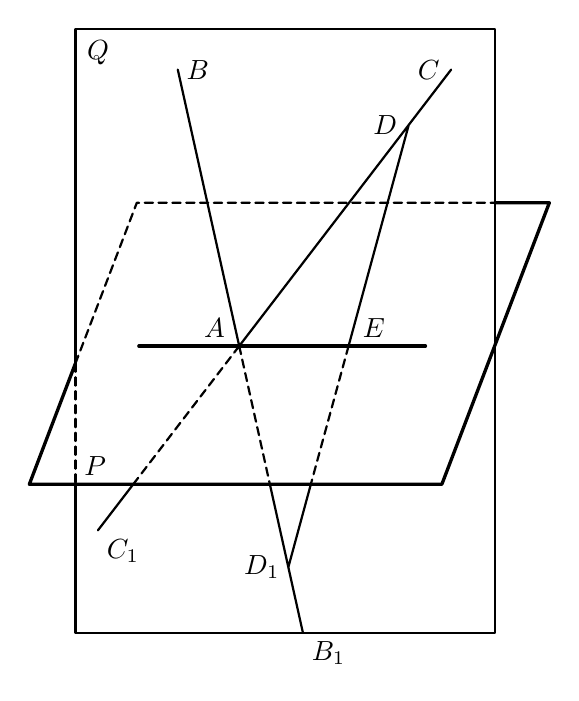
\begin{tikzpicture}[scale=1.3,line cap=round,line join=round]
    \coordinate (A) at (1.6,2.8);
    \coordinate (B) at (1,5.5);
    \coordinate (B1) at (2.2222,0);
    \coordinate (C) at (3.67,5.5);
    \coordinate (C1) at (0.22,1);
    \coordinate (D) at (3.256,4.96);
    \coordinate (D1) at (2.08,0.64);
    \coordinate (E) at (2.668,2.8);

    % Плоскость Q. Часть левого ребра скрыта плоскостью P.
    \draw[thick] (0,2.63) -- (0,5.9) -- (4.1,5.9) -- (4.1,0) -- (0,0) -- (0,1.45);
    \draw[thick,densely dashed] (0,2.63) -- (0,1.45);

    % Плоскость P. Дальняя часть контура скрыта плоскостью Q.
    \draw[very thick] (0,2.63) -- (-0.45,1.45) -- (3.58,1.45) -- (4.63,4.2) -- (4.1,4.2);
    \draw[thick,densely dashed] (0,2.63) -- (0.6,4.2) -- (4.1,4.2);

    \draw[thick] (B) -- (A) (C) -- (A) (D) -- (E);
    \draw[thick,densely dashed] (A) -- (1.9,1.45) (A) -- (0.565,1.45) (E) -- (2.3,1.45);
    \draw[thick] (1.9,1.45) -- (B1) (0.565,1.45) -- (C1) (2.3,1.45) -- (D1);
    \draw[very thick] (0.62,2.8) -- (3.42,2.8);

    \node[above left,inner sep=3pt,xshift=-2pt] at (A) {\(A\)};
    \node[right,inner sep=3pt] at (B) {\(B\)};
    \node[below right,inner sep=3pt] at (B1) {\(B_1\)};
    \node[left,inner sep=4pt] at (C) {\(C\)};
    \node[below right,inner sep=3pt] at (C1) {\(C_1\)};
    \node[left,inner sep=4pt] at (D) {\(D\)};
    \node[left,inner sep=3pt] at (D1) {\(D_1\)};
    \node[above right,inner sep=3pt,xshift=2pt] at (E) {\(E\)};
    \node[above right,inner sep=3pt] at (0,1.45) {\(P\)};
    \node[below right,inner sep=4pt] at (0,5.9) {\(Q\)};
\end{tikzpicture}

    \caption{Плоскости \(P\) и \(Q\) пересекаются по прямой \(AE\)}\label{fig:kiselev-stereo-303}
\end{figure}

Что плоскости \(P\) и \(Q\) пересекаются по прямой \(AE\) (а не касаются), следует из того, что прямые \(BB_1\) и \(CC_1\), содержащиеся в плоскости \(Q\), пересекаются с \(P\).

\kiselevparagraph{para:intersection-is-a-line} \textbf{Следствие. Пересечение двух плоскостей --- всегда прямая линия.}

Действительно, если плоскости пересекаются, то они имеют общую точку, но в таком случае они имеют и общую прямую.
% Печатная с. 275.
У плоскостей не может быть общей точки вне этой прямой, иначе плоскости слились бы в одну (\hyperref[item:plane-through-line-and-point]{см.~§~\ref*{para:plane-uniqueness-corollaries}, пункт~\ref*{item:plane-through-line-and-point}}).
